% ============================================== %
% INTRODUCTION %
% ============================================== %

\section{Introduction}
\label{introduction}

% Prolog / Background %

The need for effective visual data exploration is gaining wider recognition, where automated solutions are  provided to support users from professional data analysts in industry and science to data enthusiasts who lack formal training in data analytics.
%
The goal is to enable data-driven discoveries, wherein interesting insights are unearthed from large volumes of collected data.
%
As such, recent years have seen the introduction of many visual analytic tools such as Tableau, Qlik and Spotfire. 
%
These tools aim to provide aesthetically high-quality visualizations in terms of charts, which are essentially aggregated views of the underlying data (e.g., bar charts).
%
For instance, the commercial Tableau visualization tool presents users with aggregate charts, with the expectation that some of those charts would reveal insights that a user finds interesting. 
%
Clearly, however, manually looking for insights in each visualization is a labor-intensive and time-consuming. 

%
%
Such challenge motivated multiple research efforts that focused on automatic recommendation of visualizations based on some metrics that capture the utility of a recommended visualizations (e.g., \cite{Key2012,Viegas2007,DBLP:journals/pvldb/SellamK16,DBLP:conf/ssdbm/SellamK16, Vartak2014,Vartak2015,Ehsan2016,kandel2012profiler,DBLP:journals/tvcg/SeoS06}). 
%
For instance, recent case studies have shown that a {\em deviation-based} formulation of that utility is able to provide analysts with interesting visualizations that highlight some of the particular trends of the analyzed datasets \cite{Vartak2014, Vartak2015}.
%
Differently from Tableau's user-driven approach, in that deviation-based data-driven approach, certain views of a query result (i.e., {\em target view}) are recommended if they deviate significantly from those exhibited by a reference dataset (i.e., {\em reference view}).
%
The intuition is that a view with high deviation is expected to reveal some important insights that are very particular to the data subset under analysis. 




\begin{figure}
	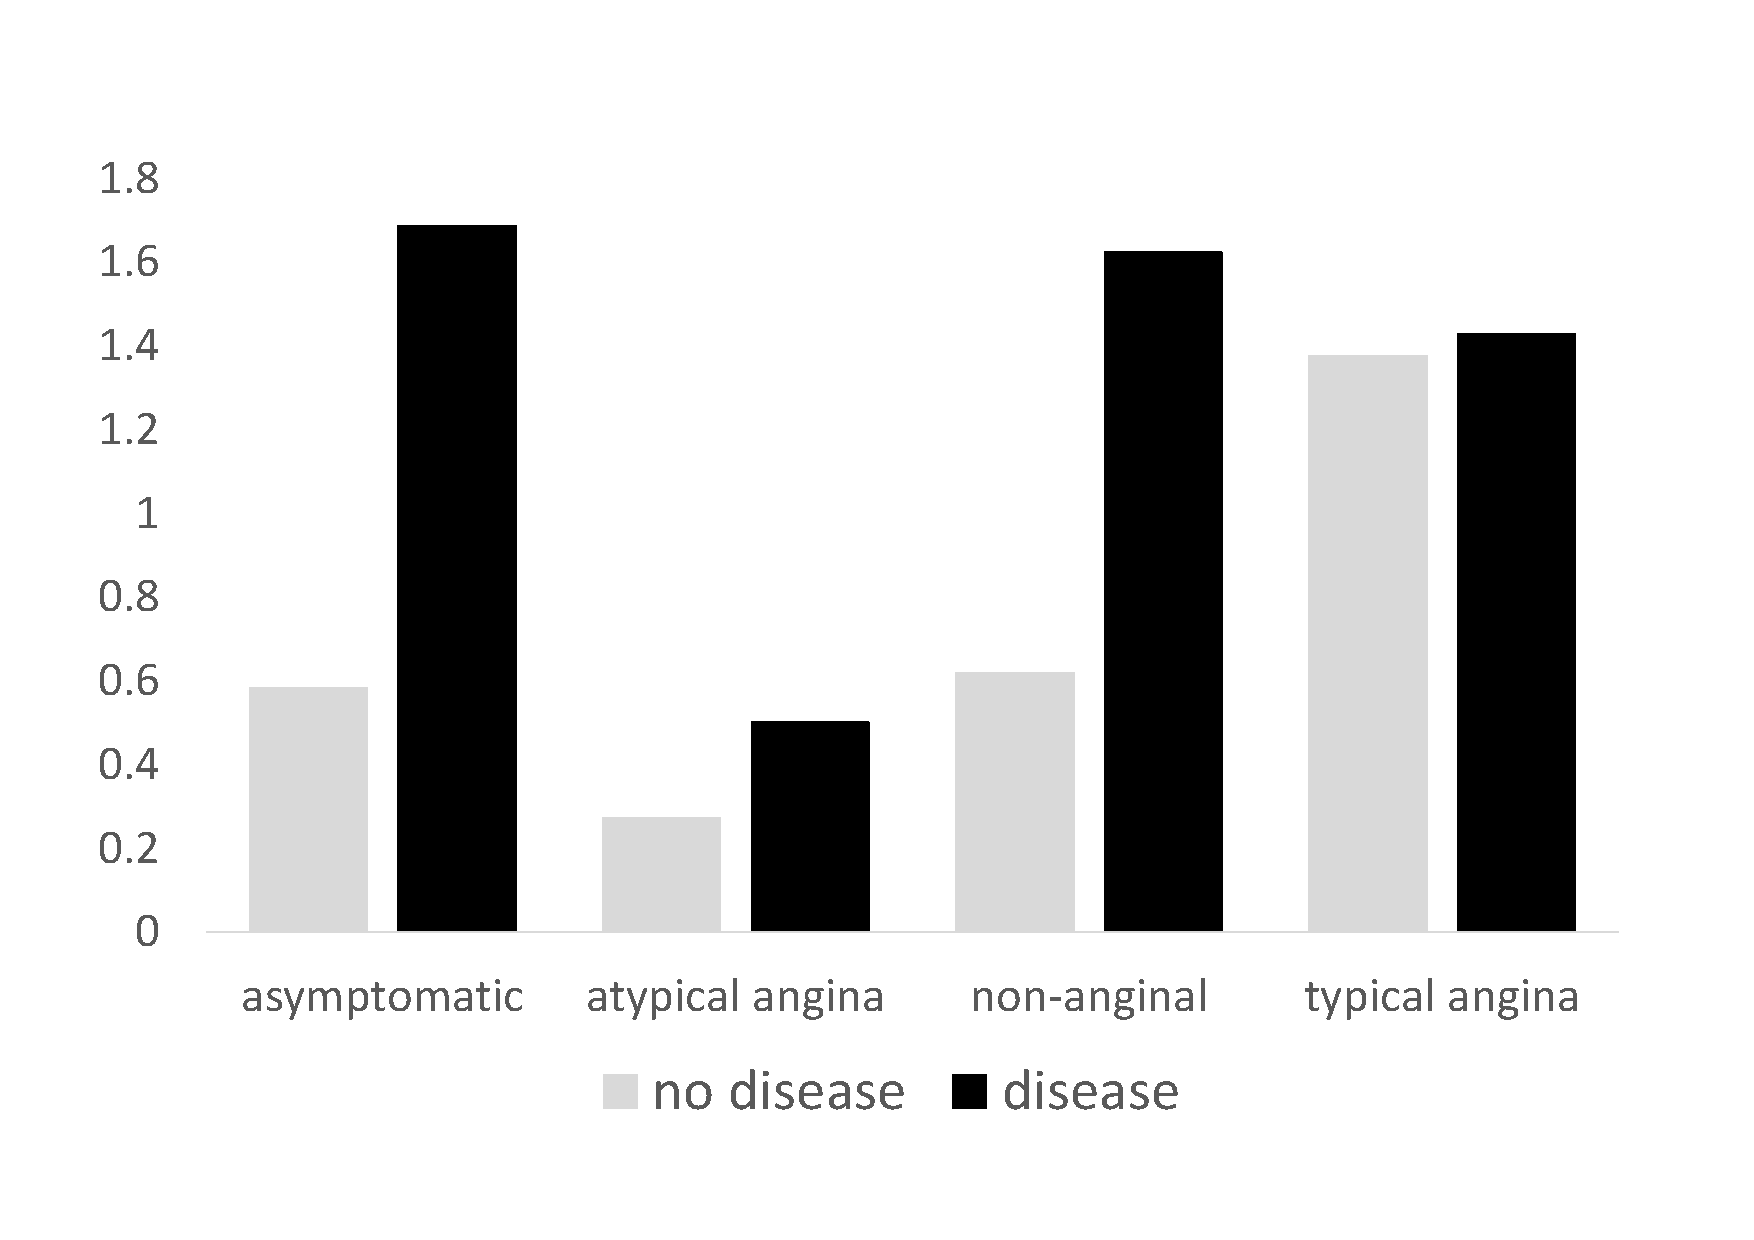
\includegraphics[width=3.0in]{figures/introduction/cp_avg_oldpeak}
	\vspace{-12pt}
	\caption{{\tt AVG}(oldpeak) vs. chest pain types}
	\label{fig:intro1}
	\vspace{-10pt}
\end{figure}

% Example /Case %


For instance, consider a data analyst trying to gain some insights into the {\em Cleveland heart disease} dataset\footnote{http://archive.ics.uci.edu/ml/datasets/heart+Disease}. 
%
Naturally, a first step in that exploratory analysis is to conduct some comparison between patients with heart disease and patients without heart disease.
%
Hence, the analyst writes an SQL query that selects patients with heart disease (i.e., {\tt disease}) as the target data subset for analysis, and the remaining patients are selected as the reference data subset (i.e., {\tt no-disease}) .

Since the analyzed data contains different dimensions (e.g., chest pain types, sex, etc.) and different measures (oldpeak, age, etc.), it is a challenging task for the analyst to manually select the combinations of dimensions and measures that reveal interesting insights.
%
Hence, to automatically recommend interesting bar chart visualizations, different SQL aggregate functions are applied on the views generated from all the possible pairwise combinations of dimensions and measures, then the most {\em important} views are presented to the analyst.
%
For this particular example, Figure \ref{fig:intro1} shows the top-1 recommended view according to the deviation-based metric \cite{Vartak2015, Vartak2014}. 
%
The figure shows that an aggregate view (i.e., bar chart) based on {\it average oldpeak} (i.e.,  pressure of the ST segment) vs. {\it chest pain types} exhibits a large deviation between the target view ({\tt disease}) and reference view ({\tt no-disease}). 
%
That is, patients with heart disease often suffer more from asymptomatic and non-angina chest pains, in comparison to those without heart disease.  

\begin{figure}
	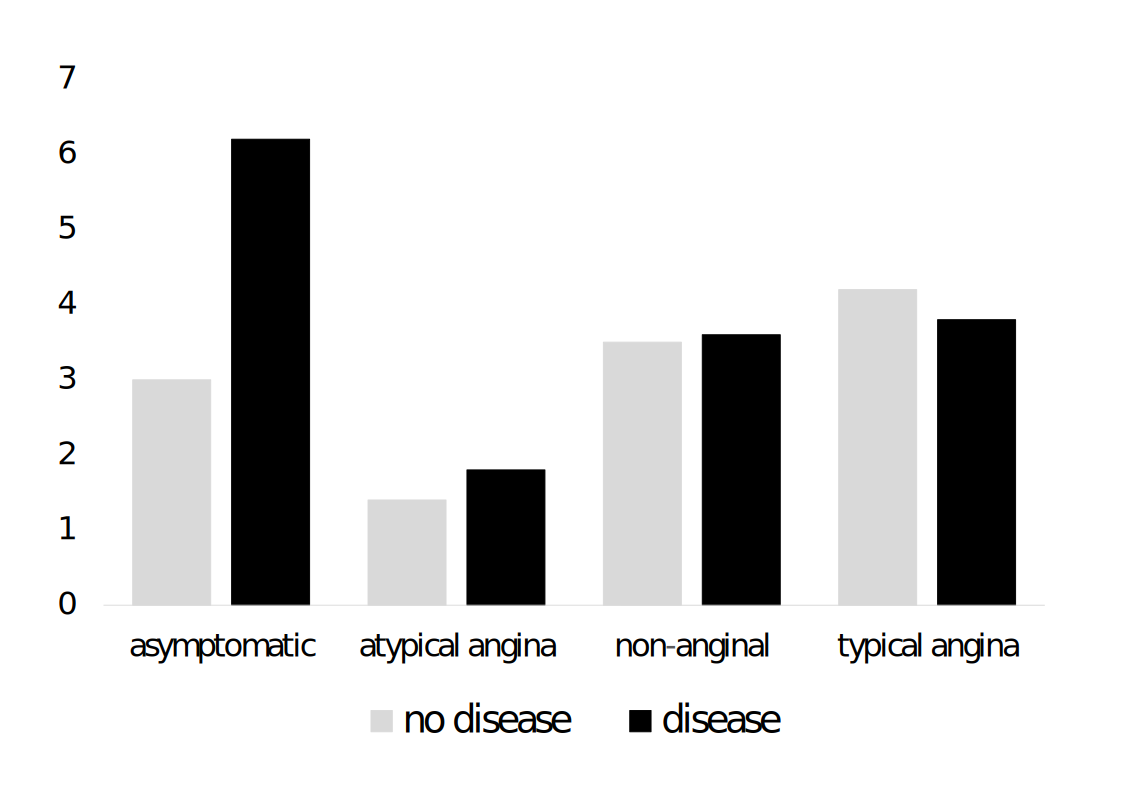
\includegraphics[width=3.0in]{figures/introduction/cp_max_oldpeak}
	\vspace{-12pt}

	\caption{ {\tt MAX}(oldpeak) vs. chest pain types}
	\label{fig:intro3}
	\vspace{-10pt}

\end{figure}

% Problem/Issue in the current solution %

While recommending views based on their importance has been shown to reveal some interesting insights \cite{Vartak2015, Vartak2014, Ehsan2016}, such approach still suffers from  a ``tunnel vision", where it often recommends similar and redundant views. 
%
For instance, Figure \ref{fig:intro3} shows the second top recommended view for the analysis described above. 
%
Comparing Figures~\ref{fig:intro3} and \ref{fig:intro1}, it is easy to see that both visualizations are based on the same dimension (i.e., {\it chest pain types}) and the same measure (i.e., {\it oldpeak}), and the only difference between them is the aggregate function (i.e., {\tt MAX} vs {\tt AVG}). 
%
Despite that similarity between the two views, they are still both recommended to the analyst due to the high deviation between the target and reference views.


% Proposing Solution %

To address that limitation, in this work we posit that employing {\em diversification} techniques in the process of view recommendation allows eliminating that redundancy and provides full coverage of the possible insights to be discovered. 
%
In fact, diversity is rapidly becoming one of the fundamental features for maximizing information gain in web search and recommendation engines (e.g., \cite{Zhang2008,Clarke2008,Rafiei2010, Yu2009}). 
%
Similarly, it is highly desirable to recommend views that reveal interesting insights, while at the same time provide the analyst with a broad scope of those insights.



To that end, we propose a hybrid objective utility function, which captures both the importance, as well as the diversity of the insights revealed by the recommended views.
%
The main goal is to select and recommend top-k views that balance the tradeoff between importance and diversity based on that hybrid objective function. 
%

In principle, traditional data diversification methods that consider both relevance and diversity can be directly applied in the context of our problem to maximize the overall objective function (e.g., \cite{Zhang2008,Rafiei2010,Yu2009}).
%
%For instance, in the context of web search, such methods are designed to recommend a set of diversified objects (e.g., web documents) that are relevant to the user needs. 
%
However, differently from assessing  relevance, evaluating the importance of a view is a computationaly expensive operation, which requires the execution of rather data-intensive queries. 
%
As such, directly applying those methods leads to a ``process-first-diversify-next" approach \cite{Zhang2008,Rafiei2010}, in which all possible data visualization are generated first via executing a large number of aggregate queries. 
%
To address that challenge and minimize the incurred query processing cost, we propose an integrated scheme called {\em DiVE}, which leverages the properties of both the importance and diversity to prune a large number of low-utility views without compromising the quality of recommendations. 
%
The main contributions of this paper are summarized as follows:

%\setlength{\leftmargini}{6pt}
\begin{itemize}
%\setlength{\itemsep}{-2pt}

	\item We formulate the problem of recommending views that are both important and diverse based on a hybrid objective function, which balances the tradeoff between the {\em content} and the {\em context} of recommended view ({\bf Section~\ref{sec:diversifying_recommended_visualizations}}). 
		
	\item We propose the novel \textit{DiVE} schemes, which employ several algorithms to select the recommended visualizations based on our hybrid ranking/objective function ({\bf Section~\ref{sec:dive_schemes}}).
	
	\item We propose novel optimization techniques that leverage the salient characteristics of our objective function to minimize the query processing cost incurred in view recommendation while maximizing the quality of recommendation ({\bf Section~\ref{sec:dive_schemes}}).
	
	\item We conduct an extensive experimental evaluation on real datasets, which compare the performance of various algorithms and illustrate the benefits achieved by \textit{DiVE} ({\bf Sections~\ref{sec:experimental_testbed} }). 
\end{itemize}


%
%}
%
%\eat{
%	+++ remove the figure with age and for the remaining two figures put a label on the x and y axis
%	
%	For instance, consider a Cleveland heart disease dataset \footnote{http://archive.ics.uci.edu/ml/datasets/heart+Disease}, which describes patients with and without a heart disease.  A data analyst might be interested in conducting some comparison between people with heart disease ({\bf disease}) and people without heart disease ({\bf no disease}). 
%	% Explanation of the example %
%	Let the target subset be the data of people with heart disease and the reference subset be the data of people without heart disease. As shown in Figure \ref{fig:intro1} {\it average oldpeak} (pressure of the ST segment) vs. {\it chest pain types} is more important view rather than Figure \ref{fig:intro2} the {\it average of age} vs. {\it chest pain types}, due to the large deviation between target view (disease) and reference view (no disease). 
%	%Figure \ref{fig:intro1} shows people with heart disease, especially who the chest pain types is asymptomatic tend to have much higher oldpeak rather than people without disease. 
%	To the contrary, Figure \ref{fig:intro2} is potentially less important view compared to Figure \ref{fig:intro1}, even there is a deviation but the deviation is very small and it is lower than Figure \ref{fig:intro1}. 
%	%Figure \ref{fig:intro2} shows that there is no significant different in term of the average age of the people with four types of chest pain.
%}

%\begin{figure}
%	\centering
%	\begin{subfigure}[b]{0.40\textwidth}
%		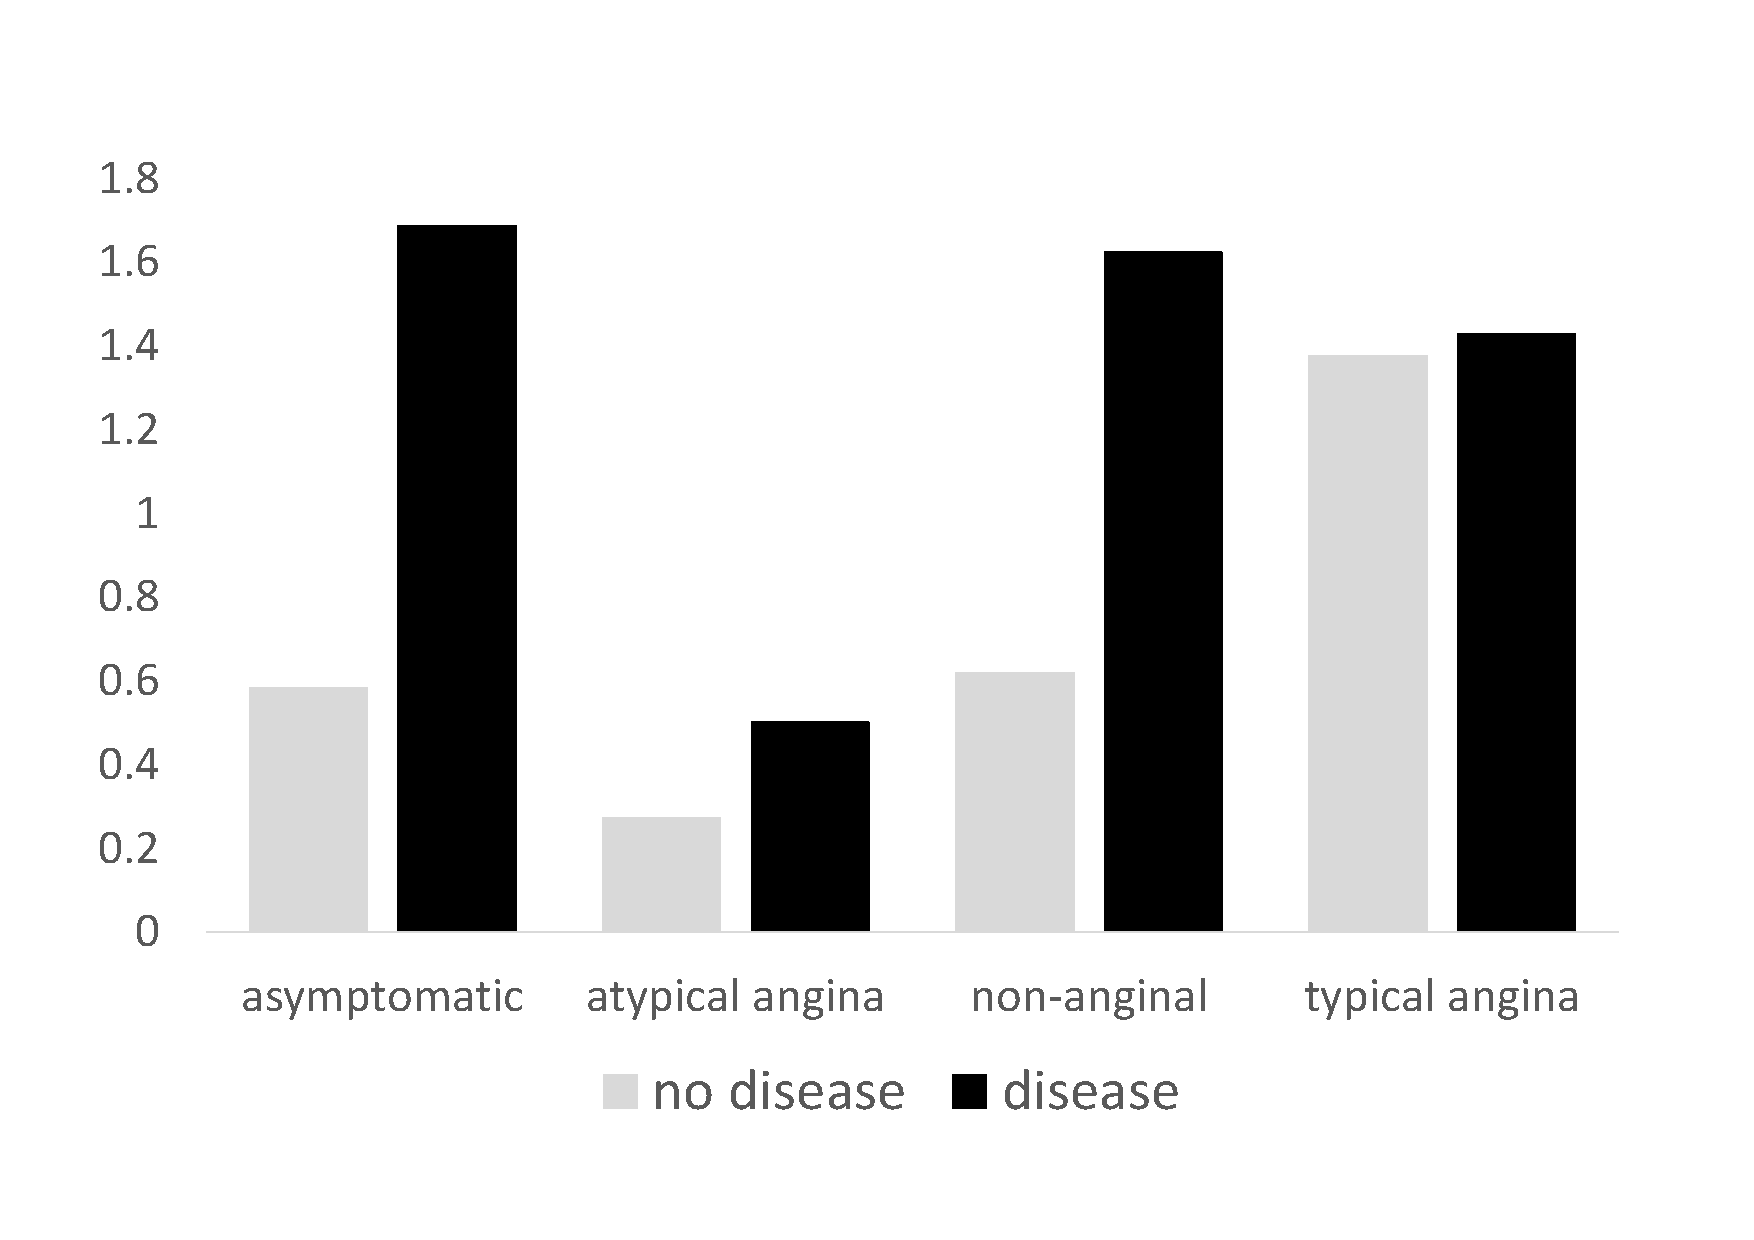
\includegraphics[width=2.5in]{figures/introduction/cp_avg_oldpeak}
%		\caption{Visualization of the avg. oldpeak vs. chest pain types}
%		\label{fig:intro1} 
%	\end{subfigure}
%	
%	\begin{subfigure}[b]{0.40\textwidth}
%		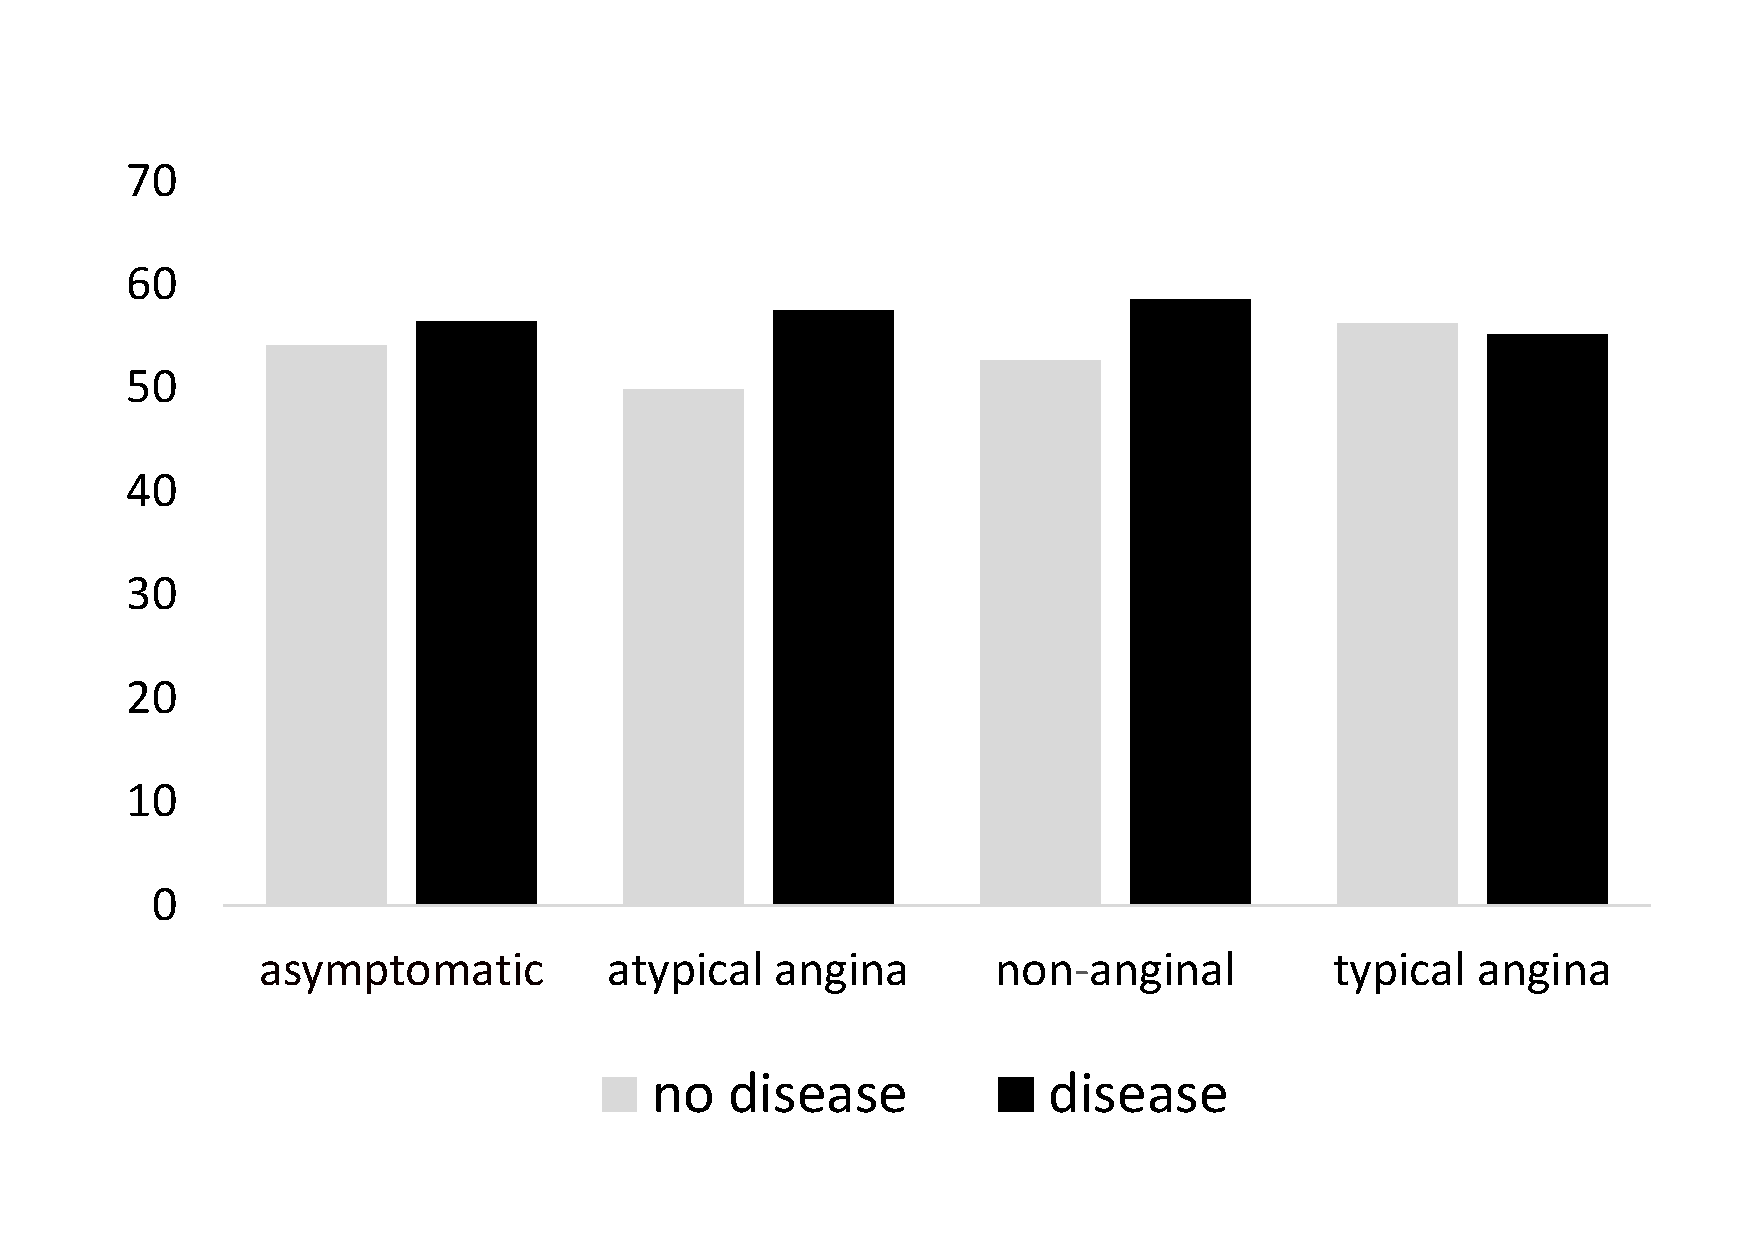
\includegraphics[width=2.5in]{figures/introduction/age_oldpeak}
%		\caption{Visualization of the average age vs. chest pain types }
%		\label{fig:intro2}
%	\end{subfigure}
%	\caption[important vs not]{Important vs. less important view.}
%\end{figure}

%In the recent years with an exponential growth of available data in various domains, there has been an increase in the number of people who trying to gain insights from the data by visual analysis ({\it data analyst}). Generaly, without any prior knowledge about the data, analyst must manually specify different combinations of attributes, measures and aggregate functions before finally generating a visualization that reveals some insights from the dataset. However, manually looking for insights in each visualization is a labor-intensive and time-consuming process. 
%
%Such challenge motivated multiple research efforts that focused on automatic recommendation of visualizations based on some metrics that capture the utility of a recommended visualizations (e.g., \cite{Key2012,Viegas2007,DBLP:journals/pvldb/SellamK16,DBLP:conf/ssdbm/SellamK16, Vartak2014,Vartak2015,Ehsan2016,kandel2012profiler,DBLP:journals/tvcg/SeoS06}. 
%
%Recent case studies have shown that {\it "a deviation-based metric"} to be effective in providing the most important visualization \cite{Vartak2014, Vartak2015}. The main goal of those works is to provide the most important visualizations ({\it top-k views}) to the analyst. In such solutions, a large number of possible views are generated and ranked according to that metric. This metric determines the deviation between the queried subset of data ({\it target view}) to the reference subset of data ({\it reference view}). The intuition behind deviation-based approach is that views that reveal substantially different trends from the reference view is judged as the important view.  

%Although the deviation-based visualization recommendation automatically provide the top-k most important views, however, it often recommends similar views and leaving the analyst with a limited amount of gained insights. 
%%
%For instance, Figure \ref{fig:intro3} provides similar insights to Figure \ref{fig:intro1}, both figures show that people with heart disease tend to have higher oldpeak values. 
%%
%Figure \ref{fig:intro3} is generated using  {\it chest pain types} as the attribute, {\it oldpeak} as the measure and {\tt MAX} as the aggregate function, whereas Figure \ref{fig:intro1}, uses same attribute and measure but uses {\tt AVG} as the aggregate function.
%%
%As shown in both figures, since those two views have a high deviation from the reference view, both views are considered as the important views and those will appear in the top-k set. 
%%
%This leads to an important observation that using "only importance" as the only criterion (e.g. a deviation-based metric) is that often deliver redundant recommended views, which leads to presents limited insights of results. 

%To address that limitation, in this work we posit that employing diversification techniques in the process of view recommendation allows eliminating that redundancy and provides concise coverage of the possible insights to be discovered. 
%%
%In fact, novelty and diversity are one of the fundamental characteristics of any effective recommendation systems \cite{Zhang2008,Clarke2008,Rafiei2010, Yu2009}. 
%%
%Specifically, it is highly desirable that a view recommendation can recommend the top-k views that are both importance and also provide new insights that has not been revealed by the other views. 

%% Lists of contributions %
%Towards designing an effective view recommendation that promotes both importance and diversity in recommended views, in this work, we propose an integrated approach called \textit{DiVE}. In particular, DiVE aims to generate top-k views that balance the tradeoff between importance and diversity. The main contributions of this paper are summarized as follows:
%
%\begin{itemize}
%	\item We formulate the problem of evaluating recommended views that are both importance and diverse ({\bf Section \ref{sec:diversifying_recommended_visualizations} }). 
%	\item We define a similarity measure to capture the distance between two visualizations ({\bf Section \ref{sec:diversifying_recommended_visualizations}}).
%	\item We present a hybrid objective function to balance the tradeoff between importance and diversity when ranking the visualizations ({\bf Section \ref{sec:diversifying_recommended_visualizations}}).
%	\item We propose the novel \textit{DiVE} schemes, that employs various algorithms to evaluate the recommended visualizations based on the hybrid ranking/objective function ({\bf Section \ref{sec:dive_schemes}}).
%	\item We present optimization techniques that leverage the hybrid objective function to substantially reduce the computational costs ({\bf Section \ref{sec:dive_schemes}}).
%	\item We conduct an extensive experimental evaluation on real datasets, which compare the performance of various algorithms and illustrate the benefits achieved by \textit{DiVE} both in terms of effectiveness and efficiency ({\bf Section \ref{sec:experimental_testbed}}). 
%\end{itemize}